\documentclass[tikz,border=5pt]{standalone}
\usetikzlibrary{positioning,ext.paths.ortho,fit,arrows.meta}
\usepackage{fourier}
\begin{document}
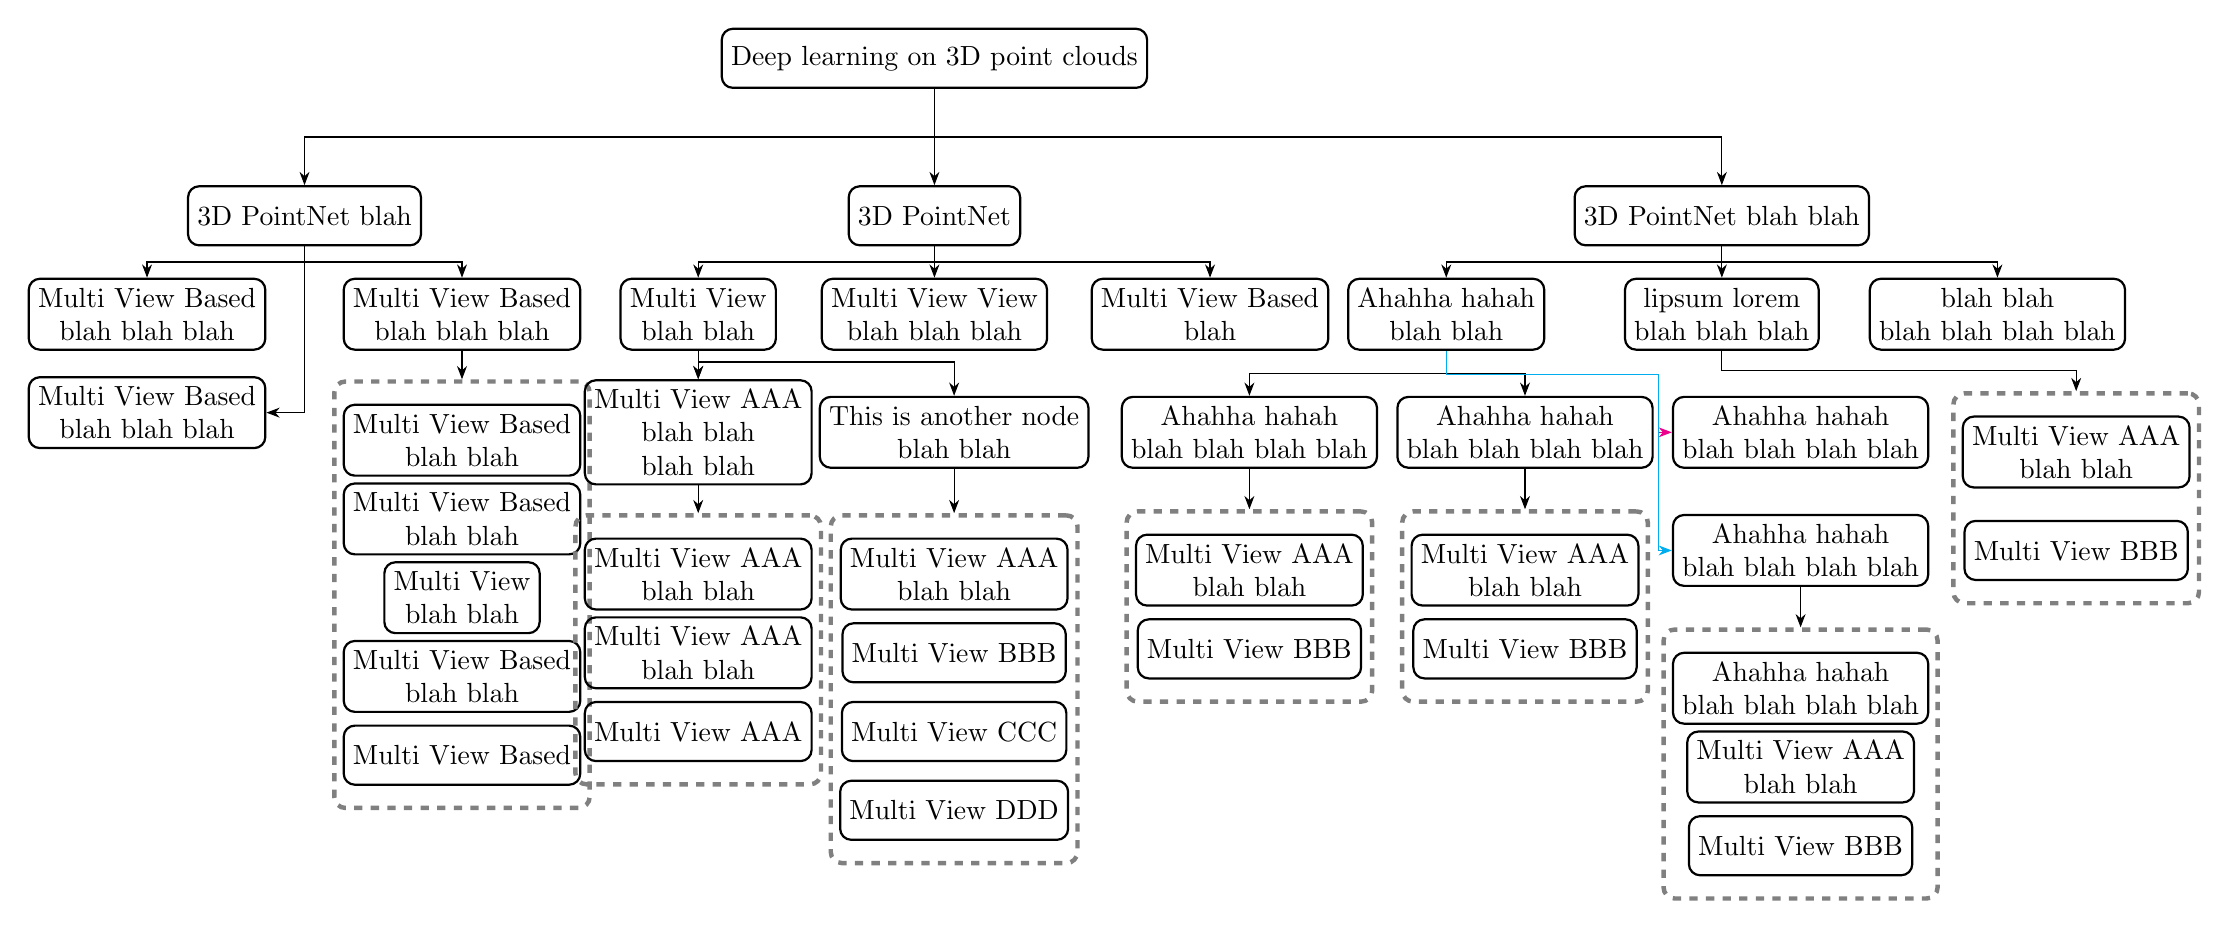
\begin{tikzpicture}[
    on grid,>=Stealth,
    % smalldist/.style={node distance=1cm}, % default
    middledist/.style={node distance=1.25cm and 2cm},
    fittedbox/.style={dashed,gray,ultra thick,inner ysep=8pt,inner xsep=3pt},
    every node/.style={draw,thick, align=center,minimum height=.75cm,rounded corners=4pt}
]
    %Root Layer
    \node[] (root) {Deep learning on 3D point clouds};
    \node[below left=2cm and 8cm of root] (L) {3D PointNet blah};
    \node[below=2cm of root,] (M) {3D PointNet} (root);
    \node[below right=2cm and 10cm of root] (R) {3D PointNet blah blah};
    \path (root) edge[->] (M);  
    \draw[->] (root) |-| (L);  
    \draw[->] (root) |-| (R);
    %Left
    \node[middledist,below left=of L] (L-11) {Multi View Based\\blah blah blah};
    \node[middledist,below right=of L] (L-12) {Multi View Based\\blah blah blah};
    \node[middledist,below =of L-11] (L-21) {Multi View Based\\blah blah blah};
    \draw[->] (L) |-| (L-11);  
    \draw[->] (L) |-| (L-12);  
    \draw[->] (L) |- (L-21);
    \node[below=1.6cm of L-12] (L-22) {Multi View Based\\blah blah};
    \node[below=of L-22] (L-32) {Multi View Based\\blah blah};
    \node[below=of L-32] (L-42) {Multi View \\blah blah};
    \node[below=of L-42] (L-52) {Multi View Based\\blah blah};
    \node[below=of L-52] (L-62) {Multi View Based};
    \node[fit=(L-22)(L-32)(L-42)(L-52)(L-62),fittedbox] (L-Tree) {} edge[<-] (L-12);
    %Middle---------------
    \node[below left=1.25cm and 3cm of M] (M-11) {Multi View\\blah blah};
    \node[middledist,below =of M] (M-12) {Multi View View\\blah blah blah};
    \node[below right=1.25cm and 3.5cm of M] (M-13) {Multi View Based\\blah};
    \draw[->] (M) |-| (M-11);  \draw[->] (M) -- (M-12);  \draw[->] (M) |-| (M-13);
    \node[below=1.5cm of M-11] (M-21) {Multi View AAA\\blah blah\\blah blah};
    \node[below=1.8cm of M-21] (M-31) {Multi View AAA\\blah blah};
    \node[below=of M-31] (M-41) {Multi View AAA\\blah blah};
    \node[below=of M-41] (M-51) {Multi View AAA};
    \node[fit=(M-31)(M-41)(M-51),fittedbox] (M-Tree1) {} edge[<-] (M-21);
    \draw[->] (M-11) -- (M-21);

    \node[right = 3.25cm of M-21] (M-22) {This is another node\\blah blah};
    \draw[->] (M-11) |-|[ratio=0.25] (M-22);

    \node[below =1.8cm of M-22] (M-32) {Multi View AAA\\blah blah};
    \node[below =of M-32] (M-42) {Multi View BBB};
    \node[below =of M-42] (M-52) {Multi View CCC};
    \node[below =of M-52] (M-62) {Multi View DDD};
    \node[fit=(M-32)(M-42)(M-52)(M-62),fittedbox] (M-Tree2) {} edge[<-] (M-22);
    \draw[->] (M-11) -- (M-21);

    %Right ---------
    \node[below left=1.25cm and 3.5cm of R] (R-11) {Ahahha hahah\\blah blah};
    \node[middledist,below =of R] (R-12) {lipsum lorem\\blah blah blah};
    \node[below right=1.25cm and 3.5cm of R] (R-13) {blah blah\\blah blah blah blah};
    \draw[->] (R) |-| (R-11);  \draw[->] (R) -- (R-12);  \draw[->] (R) |-| (R-13);
    
    \node[below left=1.5cm and 2.5cm of R-11] (R-21) {Ahahha hahah\\blah blah blah blah};
    \node[below =1.75cm of R-21] (R-31) {Multi View AAA\\blah blah};
    \node[below =of R-31] (R-41) {Multi View BBB};
    \node[fit=(R-31)(R-41),fittedbox] (R-Tree1) {} edge[<-] (R-21);

    \node[below right=1.5cm and 1cm of R-11] (R-22) {Ahahha hahah\\blah blah blah blah};
    \node[below =1.75cm of R-22] (R-32) {Multi View AAA\\blah blah};
    \node[below =of R-32] (R-42) {Multi View BBB};
    \node[fit=(R-32)(R-42),fittedbox] (R-Tree2) {} edge[<-] (R-22);

    \node[below right=1.5cm and 4.5cm of R-11] (R-23) {Ahahha hahah\\blah blah blah blah};
    \node[below=1.5cm of R-23] (R-33) {Ahahha hahah\\blah blah blah blah};
    \node[below=1.75cm of R-33] (R-43) {Ahahha hahah\\blah blah blah blah};
    \node[below =of R-43] (R-53) {Multi View AAA\\blah blah};
    \node[below =of R-53] (R-63) {Multi View BBB};
    \node[fit=(R-43)(R-53)(R-63),fittedbox] (R-Tree3) {} edge[<-] (R-33);

    \node[below right =1.75cm and 4.5cm of R-12] (R-24) {Multi View AAA\\blah blah};
    \node[below =1.25cm of R-24] (R-34) {Multi View BBB};
    \node[fit=(R-24)(R-34),fittedbox] (R-Tree4) {};
    \draw[->](R-12) |-| (R-Tree4);
    \draw[->] (R-11) |-| (R-21);
    \draw[->] (R-11) |-| (R-22);
    % four segments of arrow
    \coordinate (tmp) at (R-12.south); 
    \draw[->,magenta] (R-11) |- ([xshift=-.8cm,yshift=-.3cm]tmp) |- (R-23);% why yshift=-.3cm? Better solution?
    \draw[->,cyan] (R-11) |- ([xshift=-.8cm,yshift=-.3cm]tmp) |- (R-33);
\end{tikzpicture}

\end{document}